\subsection{Definition}

Linear programming consist of a maximisation of a linear fonction subject to linear constraints.

\subsubsection{Example}

\begin{tabular}{m{8cm}m{5cm}}
    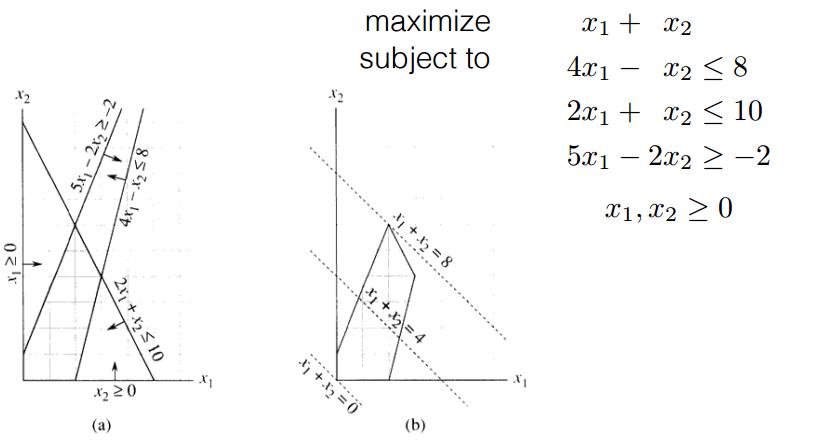
\includegraphics[width=7cm]{example1.png}
    &
    \begin{eqnarray*}
        \textrm{maximize } & x_1 + x_2 \\
        \textrm{subject to } & 4x_1 - x_2 & \leq 8 \\
                             & 2x_1 + x_2 & \leq 10 \\
                             & 5x_1 - 2x_2 & \geq -2\\
                            & x_1, x_2 \geq 0
        \end{eqnarray*}
\end{tabular}

\subsection{Polytope}

The solution space is a \textbf{polytope}. In a polytope, every point is a convex
combination of its vertices:
$$(\alpha x + (1 - \alpha)y) \in S \, \quad  with \quad \, \alpha \in
[0,1]$$

\begin{tabular}{m{8cm}m{4cm}}
    \begin{eqnarray*}
        \textrm{maximize } & c_1x_1 + ... + c_nx_n \\
        \textrm{subject to } & a_{11}x_1 + ... + a_{1n}x_n \leq b_1 \\
                             & ... \\
                             & a_{m1}x_1 + ... + a_{mn}x_n \leq b_m \\
        \end{eqnarray*}
        &
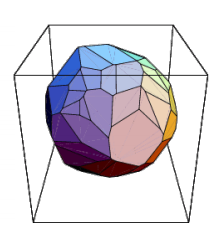
\includegraphics[width=3cm]{polytope.png}
\end{tabular}


\subsubsection{Theorem}
At least one of the points where the objective value is maximal is a vertex of the polytope.
\paragraph{Proof} : 
\begin{itemize}
    \item The maximum $x^{*}$ as a combination of the vertices of the
        polytope $v_{1},...,v_{t}$)
        $$x^{*} = \lambda_{1} v_{1} + ... + \lambda_{t} v_{t}$$

    \item Objective value at optimality can be expressed as a scalar
        product with $c$ a vector
        and the objective value at optimality can be expressed as a scalar product (c is a vector)
        $$c x^{*} = \lambda_{1} * (cv_{1}) + ... + \lambda_{t} * (cv_{t})$$
\end{itemize}

Let's assume that the maximum is not a vertex (each vertex is less good than $x^{*}$) \\
$$cx^{*} > cv_{i} \quad \forall i : 1 \leq i \leq t$$
Then we have 
\begin{align*}
cx^{*} =& \, \lambda_{1} * (cv_{1}) + ... + \lambda_{t} * (cv_{t}) \\
<& \, \lambda_{1} * (cx^{*}) + ... + \lambda_{t} * (cx^{*}) \\
<& \, (\lambda_{1} + ... + \lambda_{t}) (cx^{*}) \\
<& \, cx^{*}
\end{align*}

$\Rightarrow $ With this contradiction we can see that the maximal
$x^{*}$ must be a vertex.

\subsubsection{Algorithm}
We know that the best solution is located on a vertex of the
polytope:
\begin{enumerate}

    \item A naive approach would be to enumerate every vertices and take
        the one with the larget value. But, the problem is that the
        number of vertice grow exponentially with the number of
        inequality. 

    \item A better approach is the simplex algorithm. The idea is to
        move from one vertex to another with an improving objective
        function. We know this to be optimal thanks to the convexity of
        the polytope.
\end{enumerate}

\subsection{Simplex Algorithm}

\subsubsection{Standard and slack forms}
In order to use the simplex algorithm we need 
\begin{enumerate}
    \item Transform our linear problem  to  a \textbf{standard form}

        $\Rightarrow $ Non negativity constraint on all the
        variable and replace equality to inequality

\begin{scriptsize}
        \begin{tabular}{m{7cm}cm{7cm}}
            \begin{eqnarray*}
                \textrm{maximize } & 2x_1 - 3x_2\\
                \textrm{subject to } & x_1 + x_2 &= 7\\
                                     & x_1 - 2x_2 &\leq 4 \\
                                     & x_1 &\geq 0\\
            \end{eqnarray*}
            & $\Rightarrow$ &
            \begin{eqnarray*}
                \textrm{maximize } & 2x_1 - 3x_2 + 3x_3\\
                \textrm{subject to } & x_1 + x_2 - x_3 & \leq 7\\
                                     & -x_1 - x_2 + x_3 & \leq -7  \\
                                     & x_1 - 2x_2 + 2x_3 & \leqq 4 \\
                                     & x_1, x_2, x_3 & \geq 0\\
            \end{eqnarray*}
        \end{tabular}
\end{scriptsize}

    \item then transform standard form to a \textbf{slack form }.
        $\Rightarrow$  Introduction of basis variable in order to find a 
        \textbf{Basic Feasible Solution}

\begin{scriptsize}
        \begin{tabular}{m{7cm}cm{7cm}}
            \begin{eqnarray*}
                \textrm{maximize } & 2x_1 - 3x_2 + 3x_3\\
                \textrm{subject to } & x_1 + x_2 - x_3 & \leq 7\\
                                     & -x_1 - x_2 + x_3 & \leq -7  \\
                                     & x_1 - 2x_2 + 2x_3 & \leqq 4 \\
                                     & x_1, x_2, x_3 & \geq 0\\
            \end{eqnarray*}
            & $\Rightarrow$ &
            \begin{eqnarray*}
                \textrm{maximize } & & 2x_1 - 3x_2 + 3x_3\\
                \textrm{subject to } & x_4 =& 7 - x_1 - x_2 + x_3   \\
                                     & x_5 =&  -7 - x_1 - x_2 + x_3   \\
                                     & x_6 =&  4 - x_1 + 2x_2 - 2x_3   \\
                                     & &x_1, x_2, x_3, x_4, x_5, x_6  \geq 0\\
            \end{eqnarray*}
        \end{tabular}
\end{scriptsize}


        Slack form can be described by $(N, B, A, b, c, v)$ where

        \begin{scriptsize}
            \begin{tabular}{m{5cm}m{5cm}m{5cm}}

        \begin{itemize}
            \item $N = 
                \begin{pmatrix}
                    1 & 2 & 3
                \end{pmatrix} $
            \item $B = 
                \begin{pmatrix}
                    4 & 5 & 6
                \end{pmatrix} $
            \end{itemize}
            &

        \begin{itemize}
            \item $A = 
                \begin{pmatrix}
                    -1 & -1 & 1 \\
                    -1 & -1 & 1 \\
                    -1 & 2 & -2 
                \end{pmatrix} $
            \item $c = 
                \begin{pmatrix}
                    2 & -3 & 3
                \end{pmatrix} $
            \end{itemize}
            &
        \begin{itemize}
            \item $b =  
                \begin{pmatrix}
                    -1 & -1 & 1 \\
                    -1 & -1 & 1 \\
                    -1 & 2 & -2 
                \end{pmatrix} $
            \item $v = 0 $
            \end{itemize}
            \end{tabular}
        \end{scriptsize}
\end{enumerate}

\subsubsection{Basic Feasible Solution}
When our problem is represented as a slack we can find a BFS. 
\begin{itemize}
    \item If we can find easily a BFS:
        \begin{enumerate}
        \item We set every non basic variable to 0
        \item Then we get the value of our basis variable and 
            the objective set to 0. 
    \end{enumerate}

\item IF it's not so easy because some basics variables will be less
    than 0:
        \begin{enumerate}
        \item Put all the variables to the right such that you have
            $0 = constraints ...$
        \item Replace 0 in each constraint with a new variable
            and minimize their sum
        \item If we have a objective equal to 0, this a BFS

            Else the problem is not feasible
    \end{enumerate}

\item \textit{Basic Feasible Solution} = vertex of the standard form.

\end{itemize}

\subsubsection{Pivot}
Now the simplex algorithm will improve this BFS with the
\textbf{pivot}. 
\begin{itemize}
    \item We will increase our non
        basics variables ($x_1, x_2, x_3$) and decrease the basics one
        ($x_5, x_6, x_7$).
    \item[But] we can not decrease
        the basics ones less than 0. 
\end{itemize}

So for every non basics variables that we
will increase, we must check at what value we must stop in order to have
no basics variables under 0.

\paragraph{Example}:
\begin{scriptsize}
    \begin{enumerate}
        \item 
            \begin{tabular}{m{7cm}cm{6cm}}
                \begin{eqnarray*}
                    \textrm{maximize } & 3x_1 + x_2 + 2x_3\\
                    \textrm{subject to } &  x_4 = 30 - x_1 - x_2 - 3x_3 &
                    \textcolor{red}{x_1 \leq 30}\\
                    &  x_5 = 24 - 2x_1 - 2x_2 - 5x_3  &
                    \textcolor{red}{x_1 \leq 12} \\
                    &  x_6 = 36 - 4x_1 - x_2 - 2x_3  &
                    \textcolor{red}{x_1 \leq 9}  \\
                    & x_1, x_2, x_3, x_4, x_5, x_6  \geq 0\\
                    \\
                    \textrm{Substitute } & x_1 = 9 - \frac{x_2}{4} - \frac{x_3}{2} - \frac{X_6}{4}\\
                \end{eqnarray*} 
                & $\Rightarrow $ &
                \begin{eqnarray*}
                    \textrm{maximize } & &27 + \frac{x_2}{4} + \frac{x_3}{2} -
                    \frac{3x6}{6} \\
                    \textrm{subject to } & x_1 =&  9 + \frac{x_2}{4} + \frac{x_3}{2} -
                    \frac{3x_6}{6} \\ 
                    & x_4 =& 21 - \frac{x_2}{4} - \frac{x_3}{2} - \frac{x_6}{4} \\
                    & x_5 =& 6 - \frac{3x_2}{2} + 4x_3 + \frac{x_6}{2} \\
                    && x_1, x_2, x_3, x_4, x_5, x_6  \geq 0\\
                \end{eqnarray*} 
            \end{tabular}
        
                \vspace{-1.5cm}
            \begin{tabular}{m{7cm}cm{6cm}}
            \item \begin{tabular}{m{6cm}}
                    \begin{eqnarray*}
                    \textrm{Under constraint }& \textcolor{red}{x_3 \leq
                18 \quad x_3 \leq \frac{42}{5} \quad x_3 \leq \frac{3}{2}}\\
                    \textrm{Substitute } & x_3 = \frac{3}{2} - \frac{3x_2}{8} 
                    - \frac{x_5}{4} + \frac{X_6}{8}
                \end{eqnarray*}
                \end{tabular}

                \vspace{-1cm}
            \item \begin{tabular}{m{6cm}}
                \begin{eqnarray*}
                    \textrm{Under constraint }& \textcolor{red}{x_2 \leq
                132 \quad x_2 \leq 4 }\\
                    \textrm{Substitute } & x_3 = \frac{3}{2} - \frac{3x_2}{8} 
                    - \frac{x_5}{4} + \frac{X_6}{8}
                \end{eqnarray*}
                \end{tabular}
                & $\Rightarrow $  &
                \begin{eqnarray*}
                    \textrm{maximize } & &28 \textcolor{red}{-} \frac{x_3}{6} 
                    \textcolor{red}{-}\frac{x_5}{6} \textcolor{red}{-}
                    \frac{2x_6}{3} \\
                    \textrm{subject to } & x_1 =&  8 + \frac{x_3}{6} + \frac{x_5}{6} -
                    \frac{x_6}{3} \\ 
                    & x_2 =& 4 - \frac{8x_3}{3} - \frac{2x_5}{3} + \frac{x_6}{3} \\
                    & x_4 =& 18 + \frac{x_3}{2} + \frac{x_5}{2} \\
                    && x_1, x_2, x_3, x_4, x_5, x_6  \geq 0\\
                \end{eqnarray*} 
                \end{tabular}
    \end{enumerate}
\end{scriptsize}


\subsubsection{Cycling and degeneracy}

Sometimes an iteration will leaves the objective value unchanged
(degeneracy). This can lead to cycling leaving us the same slack form at
two different iterations. Those cycles can be avoided by breaking ties
choosing the variables with the smallest index for example (Brand's
rule). (Line 3 and 8 of the simplex algorithm).

\subsubsection{Limit of the simplex algorithm}

Most of the time the simplex algorithm performs very well. But it has
been shown that on some particular problem we get a worst case scenario
of exponential complexity. LP solving is not NP Hard, there exists other
algorithm of polynomial complexity (Ellipsoid, Interior points). Those
algorithms are not necessarily better than the simplex.

\subsection{Pseudo-code}
\begin{tiny}
\begin{tabular}{m{8cm}m{8cm}}
    \begin{lstlisting}[mathescape]
SIMPLEX(A, b, c):
    (N, B, A, b, c, b) = INITIALAZE-SIMPLEX(A, b, c)
    while some index $j \in N$ has $c_j > 0$ do
*       choose an index $e \in N$ for which $c_e > 0$
            for each index $i \in B$ do
                if $a_{ie} > 0$: $\Delta_i = b_i / a_{ie}$
                else $\Delta_i = \infty$
*           choose an index $l \in B$ that minimizes $\Delta_i$
            if $\Delta_i = \infty$: return 'undbounded'
            else (N, B, A, b, c, v) = PIVOT(N, B, A, b, c, v, l, e)

    for $i \in [1, n]$ do 
        if $i \in B$: $x_i* = b_i$
        else $x_i* = 0$

    return ($x_1*, x_2*,..., x_n*$)
    \end{lstlisting}
    &
    \begin{lstlisting}[mathescape]
PIVOT(N, B, A, b, c, v, l, e):
// Compute the coefficients of the equations for new basic variable $x_e$
    $\widehat{b_e} = b_l / a_{le}$
    for each $j \in N - \{e\}$ do
        $\widehat{a_{ej}} = a_{lj} / a_{le}$
    $\widehat{a_{el}} = l / a_{le}$

// Compute the coefficients of the remaining constraints
    for each $i \in B - \{l\}$ do
    $\widehat{b_{i}} = b_{i} - a_{ie}\widehat{b_e}$
        for each $j \in N - \{e\}$ do
            $\widehat{a_{ij}} = a_{ij} - a_{ie}\widehat{a_{ej}}$
        $\widehat{a_{il}} =  - a_{ie}\widehat{a_{el}}$

// Compute the objective
    $\widehat{v} = v + c_e\widehat{b_e}$
    for each $j \in N - \{e\}$ do
        $\widehat{c_j} = c_j - c_e\widehat{a_{ej}}$
    $\widehat{c_l} = - c_e\widehat{a_{el}}$

// Compute new sets of basic and nonbasic variables
    $\widehat{N} = N - \{e\} \cup \{l\}$
    $\widehat{B} = B - \{l\} \cup \{e\}$

    return ($\widehat{N}, \widehat{B}, \widehat{A}, \widehat{b},
    \widehat{c}, \widehat{v}$)
    \end{lstlisting}
\end{tabular}
\end{tiny}


\subsection{Integer Linear Programming (NP-Hard)}

\begin{tabular}{m{9cm}m{6cm}}
    \begin{eqnarray*}
        \textrm{maximize } & \sum_{j=1}^n c_jx_j \\
        \textrm{subject to } & \sum_{j=1}^n a_{ij}x_j \leq b_i \quad for
        \quad i=1,2,...,m \\
        & x_j \in N \quad for \quad i=1,2,...,m
        \end{eqnarray*}
    &
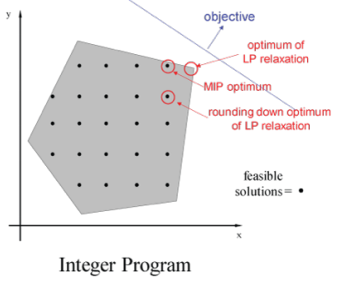
\includegraphics[width=6cm]{integerlinearprogram.png}
\end{tabular}


We can solve this using branch and bounds:

\begin{tabular}{m{12cm}m{6cm}}
    If at the optimal solution of
the linear programming relaxation, one variable is not an integer $xi =
v$, we create two branches and adding those constraints will only
decrease the upper-bound.
    &
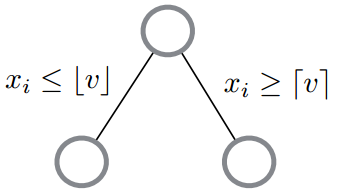
\includegraphics[width=3cm]{branch.png}
\end{tabular}



\subsection{Exam}
\begin{itemize}
    \item Formulate a linear program. 
    \item Be able to transform a LP into standard and slack form. 
    \item Explain and be able to find a initial BFS. 
    \item Apply the simplex algorithm on a small example. (be familiar with the pivoting)
    \item Explain how to detect an unbounded objective.
\end{itemize}
